\graphicspath{{introduction/fig/}}

\chapter{Introduction}
\label{chap:introduction}


In the modern day, jogging is one of the most popular physical activities. People all over the world partake in this physical activity. One would think that jogging is a simple exercise and there are no major injury or health concerns. However, there are some major concerns as jogging has a high injury rate. Over the past few years, there has been an increasing interest in this subject and many studies have been conducted on how these injuries can be analyzed. Strike patterns during running has been acknowledged as potential way of identifying injuries or risk of injury. 





\section{Problem Statement}
There are not many commercial devices that can determine a user's foot strike patterns.
\section{Objectives}
% TODO: this sucks
The objective of this project is to use a prototype wearable device that captures the pressure applied to a grid of pressure sensing resistors. The prototype has been build by a previous student and is capable of capturing the data. The device has capabilities of transmitting the data wirelessly to a mobile phone. The main object is then to use the data captured and transmit it to a smartphone. An android application will then be designed and development that can process and display this data in a useful manner. The application can then be used by medical experts to assist in medical assessments like the Gait analysis. 
\section{Scope and Limitations}

\section{Overview of the report}
\section{Section heading}

This is some section with two table in it: Table~\ref{tbl:exemplars} and Table~\ref{tbl:abx_speaker}.

\begin{table}[!h]
    \mytable
    \caption{Performance of the unconstrained segmental Bayesian model on TIDigits1 over iterations in which the reference set is refined.}
    \begin{tabularx}{\linewidth}{@{}lCCCCC@{}}
        \toprule
        Metric     & 1 & 2 & 3 & 4 & 5 \\
        \midrule
        WER (\%)                        & $35.4$ & $23.5$ & $21.5$ & $21.2$ & $22.9$ \\
        Average cluster purity (\%)       & $86.5$ & $89.7$ & $89.2$ & $88.5$ & $86.6$ \\
        Word boundary $F$-score (\%)         & $70.6$ & $72.2$ & $71.8$ & $70.9$ & $69.4$ \\
        Clusters covering 90\% of data   & 20             & 13 & 13 & 13 & 13 \\
        \bottomrule
    \end{tabularx}
    \label{tbl:exemplars}
\end{table}


\begin{table}[!h]
    \renewcommand{\arraystretch}{1.1}
    \centering
    \caption{A table with an example of using multiple columns.}
    \begin{tabularx}{0.65\linewidth}{@{}lCCr@{}}
        \toprule
        & \multicolumn{2}{c}{Accuracy (\%)} \\
        \cmidrule(lr){2-3}
        Model    & Intermediate & Output & Bitrate\\
        \midrule
        Baseline & 27.5         & 26.4   & 116 \\
        VQ-VAE   & 26.0         & 22.1   & 190 \\
        CatVAE   & 28.7         & 24.3   & 215 \\
        \bottomrule
    \end{tabularx}
    \label{tbl:abx_speaker}
\end{table}

\newpage

This is a new page, showing what the page headings looks like, and showing how to refer to a figure like Figure~\ref{fig:cae_siamese}.

\begin{figure}[!t]
    \centering
%     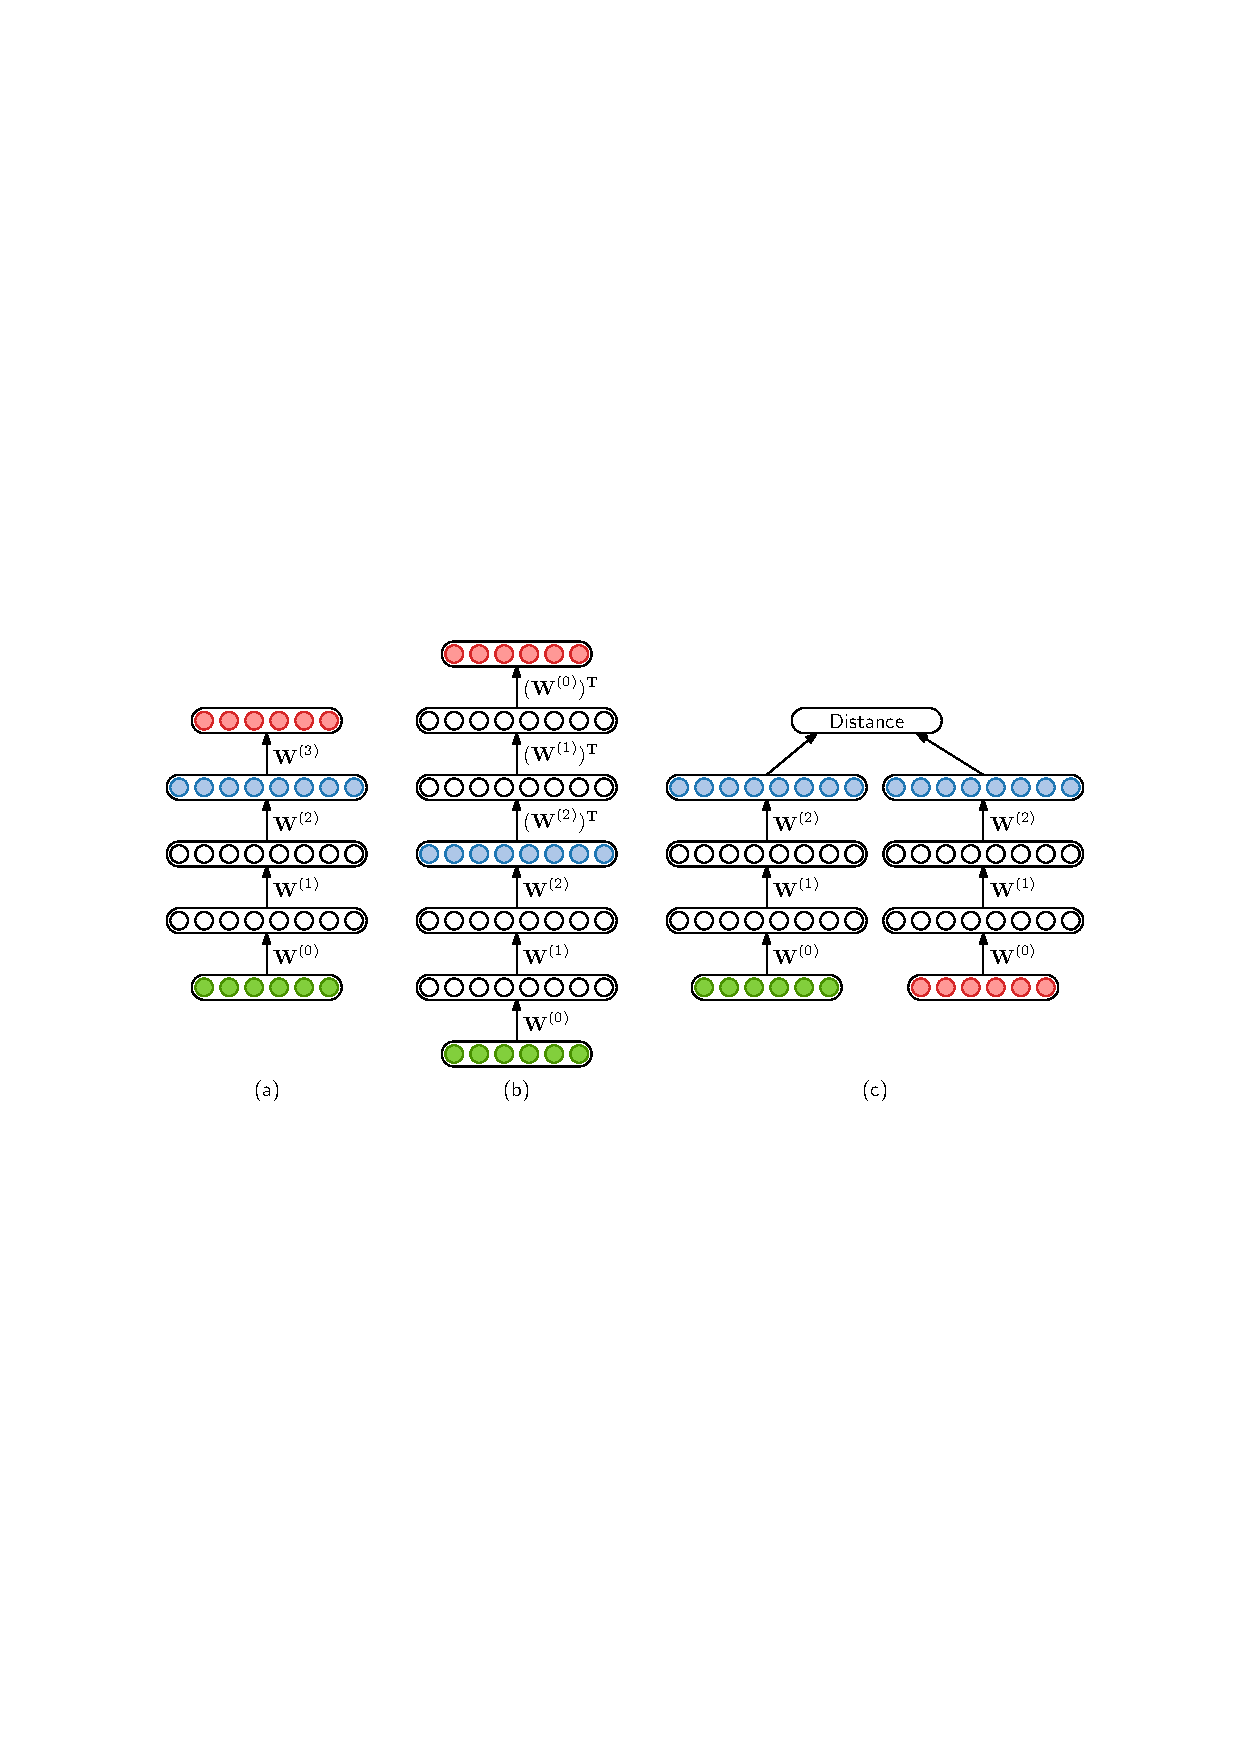
\includegraphics[width=\linewidth]{cae_siamese}
    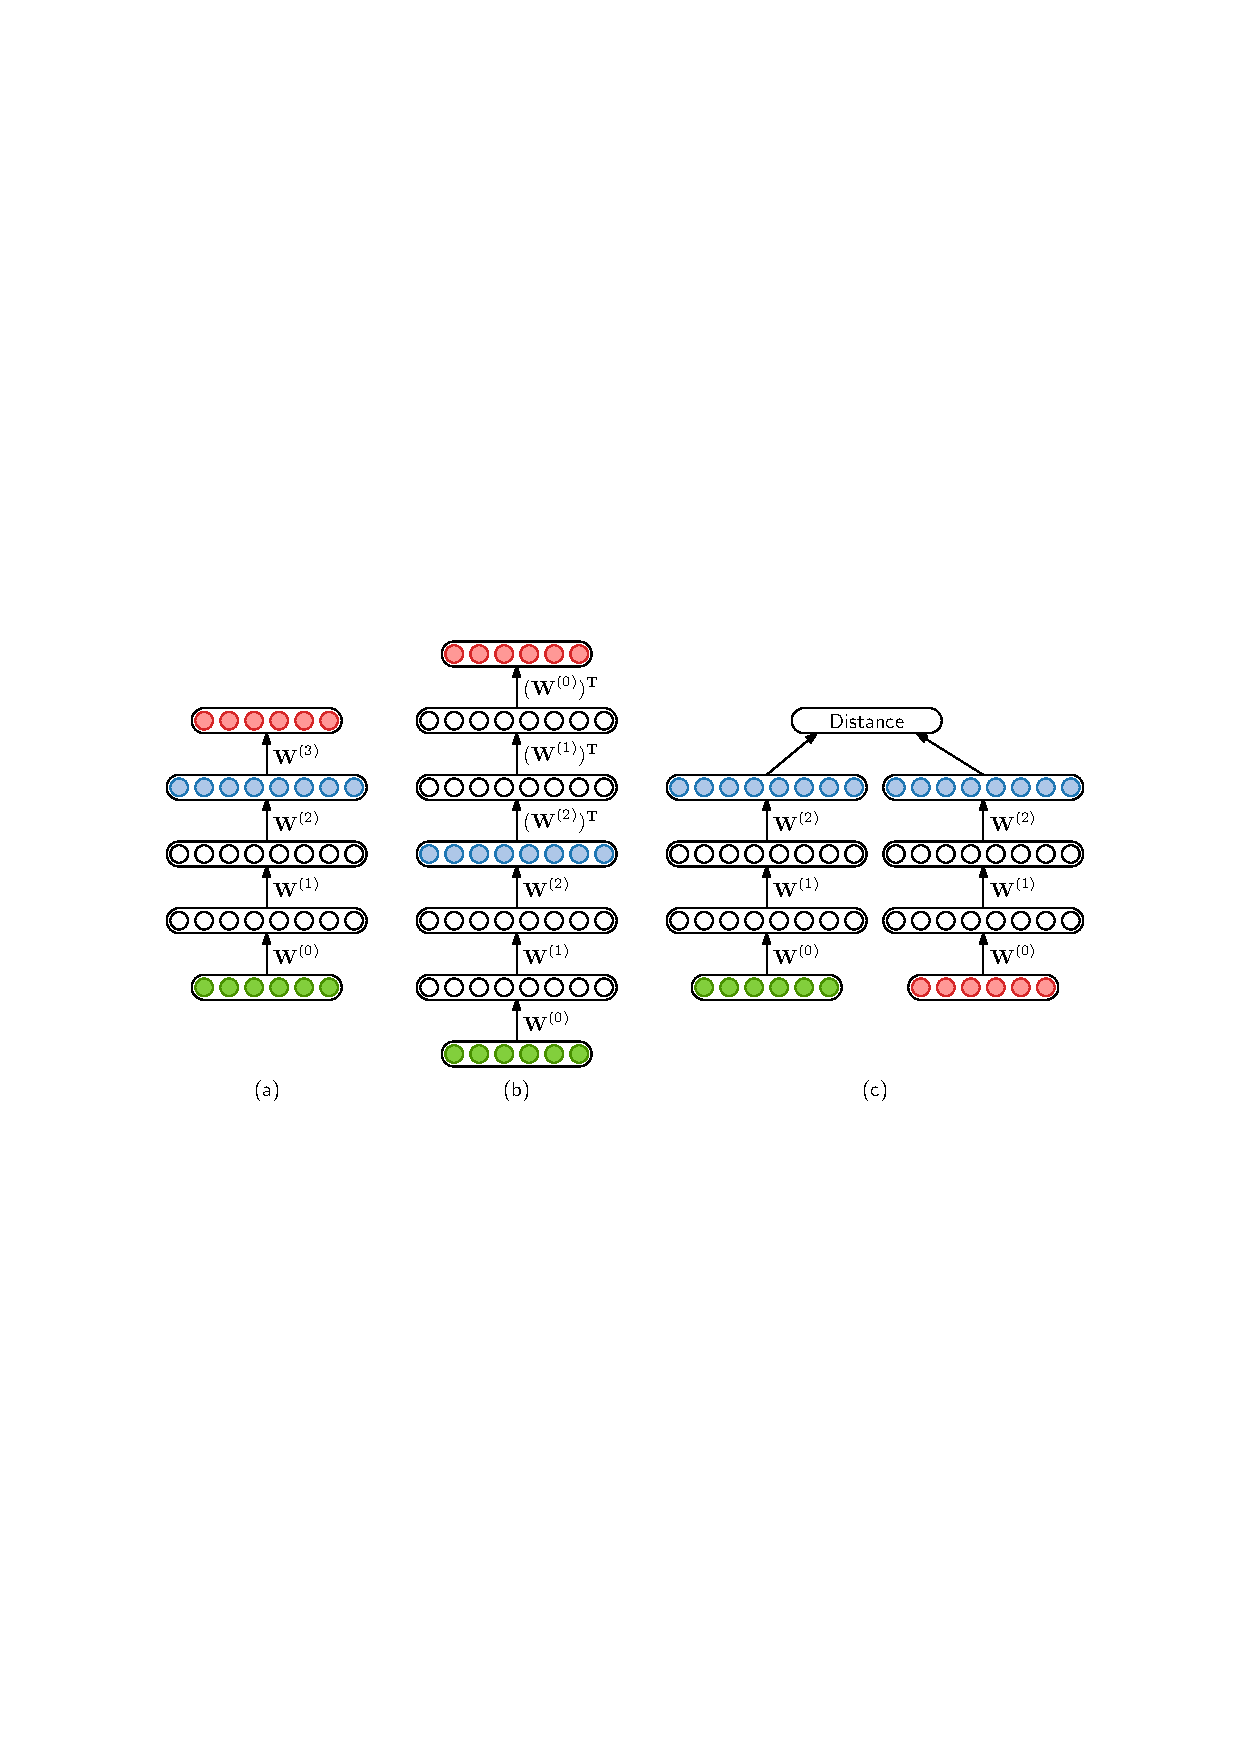
\includegraphics[width=0.918\linewidth]{cae_siamese}
    \caption[I am the short caption that appears in the list of figures, without references.]{
    (a) The cAE as used in this chapter. The encoding layer (blue) is chosen based on performance on a development set.
    (b) The cAE with symmetrical tied weights. The encoding from the middle layer (blue) is always used.
    (c) The siamese DNN. The cosine distance between aligned frames (green and red) is either minimized or maximized depending on whether the frames belong to the same (discovered) word or not.
    A cAE can be seen as a type of DNN~\cite{dahl+etal_taslp12}.
    }
    \label{fig:cae_siamese}
\end{figure}


The following is an example of an equation:
\begin{equation}
P(\vec{z} | \vec{\alpha}) = \int_{\vec{\pi}} P(\vec{z} | \vec{\pi}) \, p(\vec{\pi} | \vec{\alpha}) \, \textrm{d} \vec{\pi}
= \int_{\vec{\pi}} \prod_{k = 1}^K \pi_k^{N_k} \frac{1}{B(\vec{\alpha})} \prod_{k = 1}^K \pi_k^{\alpha_k - 1} \, \textrm{d} \vec{\pi}
\label{eq:example_equation}
\end{equation}
which you can subsequently refer to as~\eqref{eq:example_equation} or Equation~\ref{eq:example_equation}.
But make sure to consistently use the one or the other (and not mix the two ways of referring to equations).